% --------------------------------------------------------------
% This is all preamble stuff that you don't have to worry about.
% Head down to where it says "Start here"
% --------------------------------------------------------------
 
\documentclass[12pt]{article}
\usepackage[margin=1in]{geometry} 
\usepackage{amsmath,amsthm,amssymb}
\usepackage[margin=1in]{geometry} 
\usepackage{amsmath,amsthm,amssymb}
\usepackage[utf8]{inputenc}
\usepackage[T1]{fontenc} %escribe lo del teclado
\usepackage[utf8]{inputenc} %Reconoce algunos símbolos
\usepackage{lmodern} %optimiza algunas fuentes
\usepackage{graphicx}
\graphicspath{ {images/} }
\usepackage{hyperref} % Uso de links
\usepackage{float}
\date{}


\newcommand{\N}{\mathbb{N}}
\newcommand{\Z}{\mathbb{Z}}
 
\newenvironment{theorem}[2][Theorem]{\begin{trivlist}
\item[\hskip \labelsep {\bfseries #1}\hskip \labelsep {\bfseries #2.}]}{\end{trivlist}}
\newenvironment{lemma}[2][Lemma]{\begin{trivlist}
\item[\hskip \labelsep {\bfseries #1}\hskip \labelsep {\bfseries #2.}]}{\end{trivlist}}
\newenvironment{exercise}[2][Exercise]{\begin{trivlist}
\item[\hskip \labelsep {\bfseries #1}\hskip \labelsep {\bfseries #2.}]}{\end{trivlist}}
\newenvironment{problem}[2][Problem]{\begin{trivlist}
\item[\hskip \labelsep {\bfseries #1}\hskip \labelsep {\bfseries #2.}]}{\end{trivlist}}
\newenvironment{question}[2][Question]{\begin{trivlist}
\item[\hskip \labelsep {\bfseries #1}\hskip \labelsep {\bfseries #2.}]}{\end{trivlist}}
\newenvironment{corollary}[2][Corollary]{\begin{trivlist}
\item[\hskip \labelsep {\bfseries #1}\hskip \labelsep {\bfseries #2.}]}{\end{trivlist}}

\newenvironment{solution}{\begin{proof}[Solution]}{\end{proof}}
 
\begin{document}

% --------------------------------------------------------------
%                         Start here
% --------------------------------------------------------------
 
\title{Trabajo 1 Programación}
\author{Víctor Manuel Arroyo Martín\\ %replace with your name
Aprendizaje Automático}

\maketitle
\section{Ejercicio sobre la búsqueda iterativa de óptimos}
1.- El algoritmo de gradiente descendiente lo he programado según hemos dado en teoría:\\\\
Dado un dataset ($x_{n}, y_{n}$) y fijado un $w_{0}$ inicial, iteramos mientras la función f dada sea mayor que un $\varepsilon$ dado o mientras no se acaben las iteraciones máximas fijadas de antemano como sigue: 
\begin{center}
$w_{j}$ := $w_{j}$ - $\eta$ $\frac{\partial Ein(w)}{\partial w_{j}}$ \\
\end{center}
2.- a) La versión analítica del gradiente de E(u,v) = $(ue^{v}-2ve^{-u})^{2}$ es:
\begin{center}
$\nabla E(w)=\begin{bmatrix}
    2(ue^{v} - 2ve^{-u})(e^{v}+2ve^{-u}) \\
    2(ue^{v} - 2ve^{-u})(ue^{v}-2ve^{-u}) \\
\end{bmatrix}$
\end{center}
b) Tarda en alcanzarlo 10 iteraciones. El punto inicial que nos dan, el (1,1), está cerca del mínimo y además con un learning rate de 0'1 la convergencia se hace bastante rápida si lo comparamos con un learning rate de 0'01 que tardaría 65 iteraciones.\\\\
c) Coordenadas obtenidas: ( 0.04473629039778207 ,  0.023958714099141746 )
% Y este la incluye con etiqueta y pie de imagen
\begin{figure}[h]
\centering
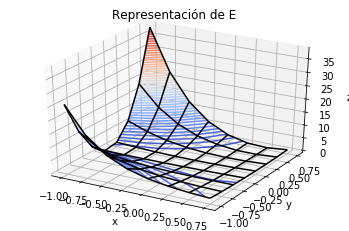
\includegraphics[scale=0.75]{Images/GraficaE1.png} 
\caption{Gráfica de la función E}
\label{etiqueta}
\end{figure}
\\
Como se ve en la figura, la superficie tiende a un mínimo mientras se acerca al (0,0) así que intuitivamente, el punto que nos sale en el algoritmo parece estar correcto. \\\\
3.- Ahora usamos f(x,y) = $(x-2)^{2} + 2(y+2)^{2} + 2sin(2\pi x)sin(2\pi y)$ \\
Las funciones fx y fy devuelven las derivadas parciales de f y gradf el gradiente que es el vector formado por ambas parciales.

\begin{figure}[h]
\centering
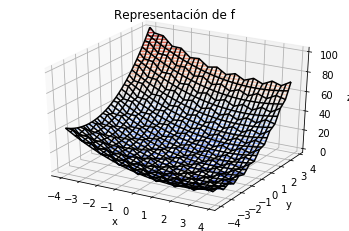
\includegraphics[scale=0.75]{Images/GraficaF1.png} 
\caption{Gráfica de la función f}
\label{etiqueta}
\end{figure}
Por la forma "rugosa" de la función podemos intuir que dependerá del punto de inicio llegar a un mínimo o a otro. Pero esto también depende del learning rate como veremos a continuación. \\\
a) Nos pedían ejecutar el gradiente descenciente para minimizar con dos learning rates: 0'1 y 0'01 y compararlos. Para ello, veamos las gráficas de decrecimiento de la función f con ambos: \\
\begin{figure}[h]
\centering
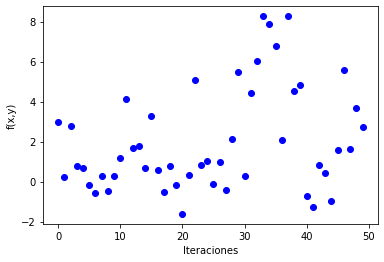
\includegraphics[scale=0.45]{Images/GraficaF01.png} 
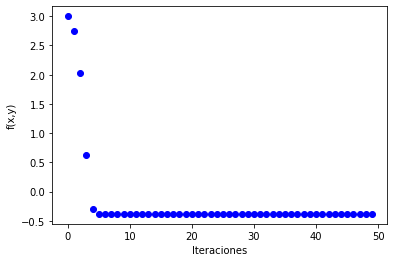
\includegraphics[scale=0.45]{Images/GraficaF001.png}
\caption{A la izquierda con $\eta$=0'1 y a la derecha con $\eta$=0'01}
\label{etiqueta}
\end{figure}
\\
Como podemos apreciar, cuando el learning rate es 0'1 se hace demasiado grande para converger al mínimo así que no debe usarse para este ejercicio. Sin embargo, para 0'01 el learning rate está bien ajustado y converge rápidamente al mínimo.
\\
b)A partir de unos puntos iniciales nos pedían obtener el mínimo y los valores donde se alcanza. Para ello, he usado el learning rate 0'01 ya que por el apartado anterior, hemos visto que no diverge. Así, la tabla de valores queda:

\begin{table}[htbp]
\begin{center}
\begin{tabular}{|l|l|l|}
\hline
Punto inicial & Valor mínimo & Punto (x,y)\\
\hline \hline
(2.1,-2.1) & -1.8200785415471563 & ( 2.2438049693647883 ,  -2.237925821486178 ) \\ \hline
(3.0,-3.0) & -0.38124949743809955 & ( 2.7309356482481055 ,  -2.7132791261667037 )\\ \hline
(1.5, 1.5) & 18.042078009957635 & ( 1.7779244744891156 ,  1.032056872669696 ) \\ \hline
(1.0, -1.0) & -0.3812494974381 & ( 1.269064351751895 ,  -1.2867208738332965 ) \\ \hline
\end{tabular}
\caption{Tabla con valores y puntos obtenidos.}
\label{tabla:sencilla}
\end{center}
\end{table}

Tal y como veíamos venir al principio, el punto mínimo también depende del valor de inicio debido a que la función presenta múltiples mínimos locales.
\\\\
4.- La conclusión que podemos sacar de estos ejercicios es que la dificultad de encontrar el máximo golobal mediante el gradiente descendiente radica no sólo en encontrar un punto inicial que sepamos que converge al mínimo global sino en usar un learning rate adecuado para ello.
\\\\
\section{Ejercicio sobre Regresión Lineal}
1.- Tras leer datos que contenían los número escritos a mano 1 y 5, nos pedían aplicarles el algoritmo de la pseudoinversa y el gradiente descendiente estocástico. Las etiquetas son -1 si es 1 y 1 si es 5. Para programarlos, se ha seguido el método propuesto en las diapositivas: \\
Primero para el SGD, se fija w como el vector 0 y se escoge un conjunto de minibatch (puntos aleatorios sin repeticiones para que estén todos igualmente representados) y se itera de la siguiente manera:
\begin{center}
$w_{j} = w_{j} - \eta \sum_{n \epsilon Minibatch}x_{nj}(h(x_{n}) - y_{n}) $ \\
Recalcular minibatch aleatorio \\
Iterar hasta el número máximo de repeticiones \\
\end{center}

Para el algoritmo de la pseoudoinversa se inicializa w al vector 0 y se usa la función que calcula pseudoinversas de numpy llamada linalg.pinv pasándole la matriz de datos x y multiplicándola por el vector de etiquetas y. Esto se le asigna a w y se devuelve. \\\\
Con un learning rate de 0.01, un máximo de 100 iteraciones y minibatch de tamaño 32, el gradiente descendiente estocástico devuelve estos valores: \\
\begin{center}
Ein:  0.21401100492129407\\
Eout:  0.25122933572588907 \\
\end{center}
Esto quiere decir que el learning rate era un poco bajo para las pocas iteraciones pero que aún así, se ajusta con bastante fidelidad a los datos incluso fuera de la muestra de entrenamiento, a diferencia de la pseudoinversa como veremos a continuación.\\ También podemos verlo gráficamente:
\begin{figure}[H]
\centering
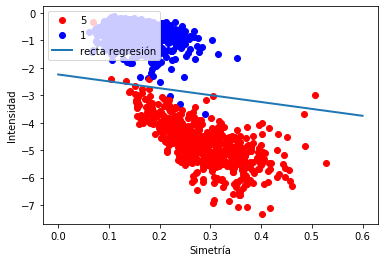
\includegraphics[scale=0.75]{Images/SGD1.png} 
\caption{Datos y recta solución para SGD}
\label{etiqueta}
\end{figure}
Para el algoritmo de la pseudoinversa, obtenemos los siguientes errores:\\
\begin{center}
Ein:  0.0791865862890038\\
Eout:  0.13095383720052578\\
\end{center}
Esto nos da una idea de que la pseudoinversa se ajusta muy bien (quizás demasiado) a los datos de entrenamiento y a la hora de hacer tests fuera de éstos, su error sube bastante.
\begin{figure}[H]
\centering
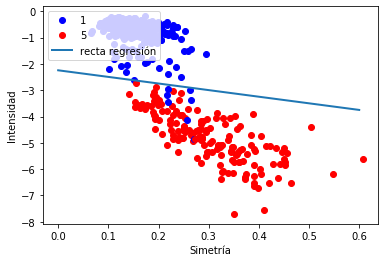
\includegraphics[scale=0.75]{Images/Pseudoinversa.png} 
\caption{Datos y recta solución para pseudoinversa}
\label{etiqueta}
\end{figure}
2.- En este apartado, nos piden hacer un experimento con 1000 puntos repartidos uniformemente en el cuadrado [-1,1]x[-1,1].\\
a) Primero calculamos aleatoriamente pero de forma uniforme estos puntos, quedando la representación como sigue:
\begin{figure}[H]
\centering
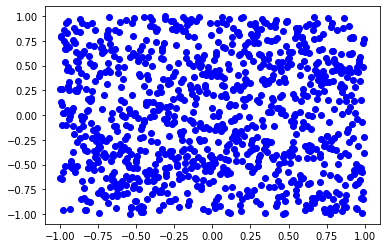
\includegraphics[scale=0.65]{Images/1000N1.png} 
\caption{Nube de puntos}
\label{etiqueta}
\end{figure}
b) Ahora asignamos etiquetas según el signo de la función $f(x_{1},x_{2})=(x_{1} - 0,2)^{2} + x _{2}^{2} - 0,6)$ en el cuadrado y añadiéndole un ruido (esto es, cambiar las etiquetas) a un 10$\%$ de la muestra. Así, la nube de puntos queda:
\begin{figure}[H]
\centering
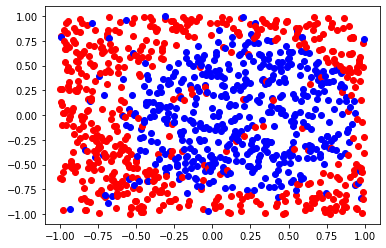
\includegraphics[scale=0.65]{Images/1000N2.png} 
\caption{Datos con sus etiquetas y ruido. Etiqueta -1 azul y 1 rojo}
\label{etiqueta}
\end{figure}
Como podemos intuir en la representación de los puntos, un modelo lineal no sería el más adecuado para este problema, como veremos en el siguiente apartado. \\
c) Ahora nos piden ajustar un modelo de regresión lineal lineal a los puntos obtenidos mediante gradiente descendiente estocástico. Con 100 iteraciones, un learning rate de 0.1 y un minibatch de 32, he conseguido un error dentro de la muestra de 0.9206097292765354. \\
Como hemos previsto antes, este modelo tiene mucho error incluso con los datos de entrenamiento. De hecho, gráficamente se puede ver:
\begin{figure}[H]
\centering
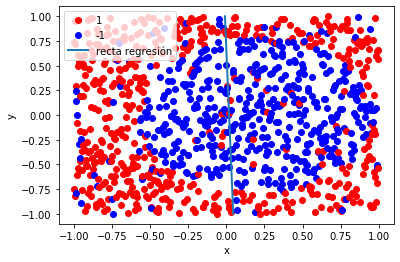
\includegraphics[scale=0.65]{Images/1000NSGD.png} 
\caption{Datos de entrenamiento y solución}
\label{etiqueta}
\end{figure}
d) En este apartado nos piden repetir el experimento anterior 1000 veces con nuevos puntos para entrenamiento y nuveos para test. Haciendo los errores medios con 100 iteraciones, un learning rate de 0.1 y un minibatch de 32, he conseguido errores medios de:
\begin{center}
Ein media:  0.9283443998809577\\
Eout media:  0.9329690185448061
\end{center}
Siguen siendo muy altos, lo cual solo reafirma lo ya dicho en el apartado anterior.\\\\
e) Valorando los errores fuera y dentro de la muestra de entrenamiento, ya hemos visto que un modelo de regresión lineal es muy malo para predecir en este caso. Un modelo con una forma gráfica de elipse habría sido mucho mejor. De hecho, eso es lo que nos piden en los dos últimos apartados. \\\\
$\bullet$Ahora nos piden hacer los mismos experimentos que en el apartado 2.- pero con el vector de características $\Phi_{2}(x)=(1,x_{1},x_{2},x_{1}x_{2},x_{1}^{2},x_2^{2})$.\\
Así, tras crear el nuevo vector de pesos ŵ a partir de los datos y sus etiquetas con un 10$\%$ de ruido, la representación gráfica queda:
\begin{figure}[H]
\centering
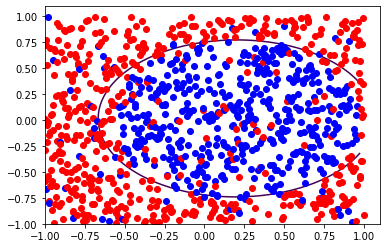
\includegraphics[scale=0.65]{Images/1000NFin.png} 
\caption{Datos de entrenamiento y recta solución}
\label{etiqueta}
\end{figure}
Visualmente se puede apreciar que se ajusta mejor a los datos que el modelo lineal. De hecho, el error dentro de la muestra es mucho menor, es de 0.5935351071569172.\\
Ahora tras repetir el experimento mil veces con nuevos datos, los errores que lanza esta nueva característica son:\\
\begin{center}
Ein media:  0.5854293055159135\\
Eout media:  0.5900846135487273
\end{center}
$\bullet$A la vista de los errores medios de ambas propuestas, el modelo con la segunda característica es mucho mejor por tener un error dentro y fuera de la muestra mucho menores que la primera. De hecho se puede hasta intuir gráficamente.
\section{BONUS}
En este ejercicio se pide programar el método de Newton que encuentra máximos relativos (el de las diapositivas) y realizar el procedimiento de la sección 1 ejercicio 3 con la misma función.\\
El método se ha programado siguiendo las diapositivas: la variación que sufre w en cada iteración viene dada por la matriz Hessiana multiplicada por el gradiente del error en el w actual, todo eso cambiado de signo.\\\\
$\bullet$Primero generamos gráficas de cómo crece el valor de la función para el punto inicial (1,-1) con dos learning rates.:\\
\begin{figure}[H]
\centering
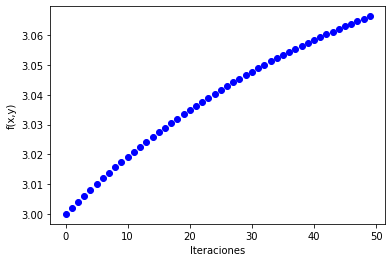
\includegraphics[scale=0.45]{Images/MN1-1001.png} 
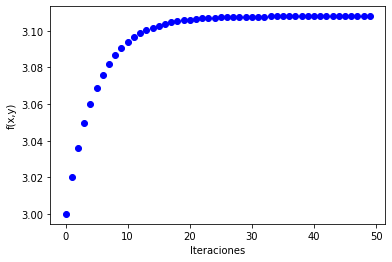
\includegraphics[scale=0.45]{Images/MN1-101.png} 
\caption{Learning rate de 0.01 a la izquierda y 0.1 a la derecha}
\label{etiqueta}
\end{figure}
Ahora para una serie de puntos iniciales se pedía dar el punto donde se alcanza el máximo, una gráfica de crecimiento de la función y el valor máximo. Para todos he usado un learning rate de 0.1 excepto para el (1.5,1.5) que he usado 0.01 pues sólo así converge:\\
\begin{figure}[H]
\centering
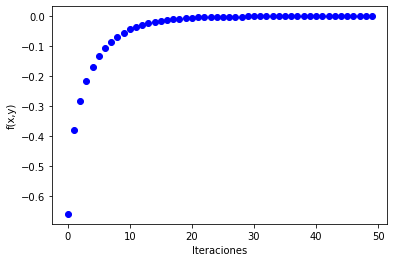
\includegraphics[scale=0.45]{Images/MN21.png} 
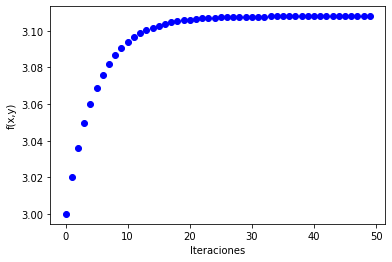
\includegraphics[scale=0.45]{Images/MN3.png} 
\caption{Punto inicial (2.1,-2.1) izquierda, (3.0,-3.0) derecha}
\label{etiqueta}
\end{figure}
Para el punto (2.1,-2.1) da un valor máximo de $-9.304464461733982\cdot 10^{-6}$ alcanzado en el punto (x,y) = ( 2.0003480109559346 ,  -2.00035204598058 ). \\
Para el punto (3.0,-3.0) da un valor máximo de 3.1079767229661335 alcanzado en el punto (x,y) = ( 3.053672597180933 ,  -3.028291762643699 ) \\

\begin{figure}[H]
\centering
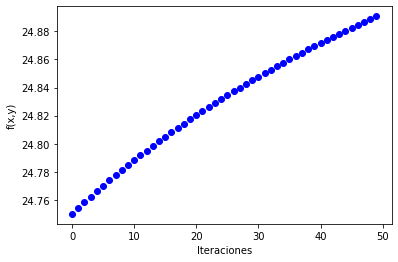
\includegraphics[scale=0.45]{Images/MN15.png} 
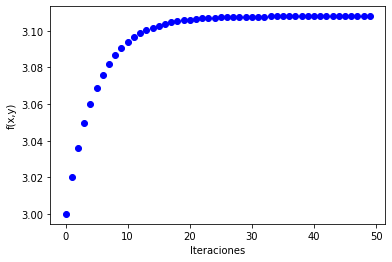
\includegraphics[scale=0.45]{Images/MN1-101.png} 
\caption{Punto inicial (1.5,1.5) izquierda, (1.0,-1.0) derecha}
\label{etiqueta}
\end{figure}
Para el punto 1.5,1.5) da un valor máximo de 24.892748286747203 alcanzado en el punto (x,y) = ( 1.4270267930033473 ,  1.5076223435327116 ). \\
Para el punto (1.0,-1.0) da un valor máximo de 3.1079767229661335 alcanzado en el punto (x,y) = ( 0.9463274028190676 ,  -0.9717082373563009 ) \\\\
$\bullet$Como comparación con el algoritmo del ejercicio 3, podemos decir que el método de Newton encuentra máximos y el otro mínimos y que ambos dependen de los puntos de inicio y del learning rate para converger a su objetivo o no.


% --------------------------------------------------------------
%     You don't have to mess with anything below this line.
% --------------------------------------------------------------
 
\end{document}